\chapter[Real-World Performance-Bug Understanding]{Real-World Performance-Bug Understanding}
\label{chap:study}

Empirical studies on functional bugs have successfully guided the design of functional software testing, 
bug detection, and failure diagnosis. 
Poor understanding of performance bugs is part of the causes of today's performance-bug problems. 
The lack of empirical studies on performance bugs has severely 
limited the design of performance-bug avoidance, testing, detection, and fixing tools.

This chapter presents our comprehensive study of real-world performance bugs, 
based on 110 bugs randomly collected from the bug databases of five representative 
open-source software suites (Apache, Chrome, GCC, Mozilla, and MySQL). 
Following the lifetime of performance bugs, our empirical study is performed in 4 dimensions: 
the root-cause of performance bugs, how performance bugs are introduced, 
how to expose performance bugs and how to fix performance bugs. Our findings and implications can guide future research in this area, 
and have already inspired our own performance-bug detection and performance failure diagnosis work. 

\section{Introduction}
\label{sec:3_introduction}

Performance bugs~\citep{s2e,perf.fse10,rily.perftest,perfantipattern} 
are software implementation mistakes that can cause slow execution.
The patches for performance bugs are often not too complex.
These patches can preserve the same functionality, and achieve significant performance improvement. 
Performance bugs cannot be optimized away by compiler optimization. 
Many of them escape from testing process and manifest in front of end users~\citep{xiao13:context}.
Performance bugs are common and severe. 
Mozilla developers have to fix 5 to 50 performance bugs each month in the last 10 years. 
Performance bugs have already caused several highly publicized failures, 
like the slow affordable care act system~\citep{ACA-health}.
Fighting performance bugs is solely needed.  

There are many misunderstanding of performance bugs, 
such as ``performance is taken care of by compilers and hardware'' and 
``profiling is sufficient to solve performance problems''. 
These wrong perceptions are partly the causes of today's performance-bug problem~\citep{lies}. 
The lack of understanding of performance bugs has severely limited the research and tool building in this area. 

There are many empirical studies on functional bugs~\citep{chou01empirical,characteristics.asplos08, 10yearlinux,emmett.ppopp10,
sullivan92comparison,Lu.study.fast}. 
Many of them are conducted along the following dimensions: 
root causes of functional bugs, 
how functional bugs are introduced, how to expose functional bugs, 
and how to fix functional bugs. 
These studies have provided guidance for functional-bug detection, 
functional failure diagnosis, functional-bug avoidance, and software testing. 
It is feasible and necessary to conduct similar studies on performance bugs for the following reasons: 

Firstly, it is feasible to sample performance-bug reports in the real world to conduct the empirical study. 
There are well-known open-source software with long well maintained bug databases. 
For some of them, developers explicitly mark certain bug reports in their bug databases as performance bugs. 
For example, Mozilla developers use ``perf'' tag to mark performance bugs. 
It is fairly easy for us to collect enough performance bugs in order to conduct the study.

Secondly, it is reasonable to understand whether techniques designed for functional bugs still work for performance bugs, 
before designing new techniques for performance bugs. 
In order to make this clear, 
it is necessary to follow the study dimension conducted on functional 
bugs to perform a similar empirical study for performance bugs. 

Finally, performance bugs are different from functional bugs. 
For example, performance bugs do not have failure symptoms, 
like crash or segmentation fault. 
We cannot directly leverage experience gained from combating functional bugs. 
It is necessary to understand the unique features and bug patterns for performance bugs.

This chapter makes the first, to the best of our knowledge,
comprehensive study of real-world performance bugs
based on \allbugs bugs randomly collected from the bug databases of five
representative open-source software suites (Apache, Chrome, GCC,
Mozilla, and MySQL). Our study has made the following findings.

{\bf Guidance for bug avoidance.\ }
Two thirds of the studied bugs are
introduced by developers' wrong understanding of workload
or API performance features.  
More than one quarter of the bugs arise from previously correct
code due to workload or API changes. 
To avoid performance bugs,
developers need performance-oriented
annotation systems and change-impact analysis.

{\bf Guidance for performance testing.\ } 
Almost half of the studied bugs require inputs with {\bf both} {special}
features and large scales to manifest. 
New performance-testing schemes that combine the input-generation techniques 
used by functional testing~\citep{KLEE,dart} with a consideration towards large 
scales will significantly improve the state-of-the-art.

{\bf Guidance for bug detection.\ } Recent works
~\citep{s2e,BloatFSE2008,perf.fse10,jolt,XuBloatPLDI2009,XuBloatPLDI2010}
have demonstrated the potential of performance-bug detection. 
Our study found common root causes and structural patterns of real-world
performance bugs that can help improve the coverage and accuracy 
of performance-bug detection.

{\bf Guidance for bug diagnosis.\ } 
The root-cause patterns and fix strategies for performance bugs are 
highly correlated. It is feasible to propose fix strategies automatically, based on identified root causes. 

{\bf Comparison with functional bugs.\ }
Performance bugs tend to hide for much longer time in software 
than functional bugs.
Unlike functional bugs, performance
bugs cannot all be modeled as rare events, because a 
non-negligible portion of them can be triggered by
almost all inputs.

{\bf General motivation\ }
(1) Many performance-bug patches are small.  The fact that we can
achieve significant performance
improvement through a few lines of code change motivates
researchers to pay more attention to performance bugs.
(2) A non-negligible portion of performance bugs in multi-threaded
software are related to synchronization.
Developers need tool support to avoid over-synchronization traps.

\section{Methodology}
\label{sec:3_meth}

This section describes how we collect performance bugs from the real world. 

{\bf Applications}
We chose five open-source software suites to examine: Apache, Chrome, GCC, 
Mozilla, and MySQL. These popular, award-winning software suites 
\citep{halloffame} are all large-scale and mature, with millions of lines of 
source code and well maintained bug databases.

\begin{table}[h!]
\centering
\scriptsize
\begin{tabular}{@{\hspace{3pt}}l@{\hspace{3pt}}@{\hspace{3pt}}c@{\hspace{3pt}}}
\toprule
Application Suite Description (language) &    \# of Bugs        \\
\midrule                            
{\bf Apache Suite} 	                 & 25              \\
%\cline{1-1}
{HTTPD:	Web Server (C)	}                & \\
{TomCat:  Web Application Server (Java)} & \\
{Ant:	Build management utility (Java)} & \\
%\hline
%JMeter	& Load test utility (Java) & \\
\midrule                            
{\bf Chromium Suite} Google Chrome browser (C/C++) &  10 \\
\midrule
%\multicolumn{2}{|l|}
{\bf GCC Suite}  GCC \& G++ Compiler (C/C++)   & 11  \\
\midrule
{\bf Mozilla Suite} & 36  \\
%\cline{1-1}
{Firefox: Web Browser (C++, JavaScript)}& 	\\
{Thunderbird: Email Client (C++, JavaScript)}& \\
\midrule
{\bf MySQL Suite}    & 28 	\\
%\cline{1-1}
{Server: Database Server (C/C++)}&  	\\
%\cline{1}
{Connector: DB Client Libraries (C/C++/Java/.Net)}&  	\\
\midrule
{\bf Total}	  & \allbugs  \\
\bottomrule
\end{tabular}
\caption{Applications and bugs used in the study.}
\label{tab:3_app_allbug}
\end{table}

As shown in Table~\ref{tab:3_app_allbug},
these five suites provide a good coverage of various types of software, 
such as interactive GUI 
applications, server software, command-line utilities, compilers,
and libraries.
They are primarily written in C/C++ and Java. 
Although they are all open-source software, Chrome is 
backed up by Google
and MySQL was acquired by Sun/Oracle in 2008.
Furthermore, the Chrome browser was first released
in 2008, while the other four
have had 10--15 years of bug reporting history.
From these applications, we can observe both traditions and new software
trends such as web applications.

{\bf Bug Collection}
GCC, Mozilla, and MySQL developers {\it explicitly} mark certain reports in
their bug databases as performance bugs using special tags, which are 
{\it compile-time-hog}, {\it perf}, and {\it S5} respectively.
Apache and Chrome developers do not use any special tag to mark performance 
bugs. Therefore, we searched their bug databases using
a set of performance-related keywords 
(`slow', `performance', `latency', 
`throughput', etc.).

From these sources, we {\it randomly} sampled \allbugs fixed bugs that
have sufficient documentation.
Among these bugs, 44 were reported after 2008, 39 were
reported between 2004 and 2007, and 27 were reported before 2004.
41 bugs came from server applications and 69 bugs came
from client applications. 
The details are shown in Table~\ref{tab:3_app_allbug}.


{\bf Caveats}
Our findings need to be taken with the methodology in mind. 
The applications in our study cover representative and important software 
categories, workload, development background, and programming languages.
Of course, there are still uncovered categories, such as scientific
computing software and distributed systems.

The bugs in our study are collected from five bug databases without bias. 
We have followed the decisions made by developers about what are performance 
bugs,
and have not intentionally ignored any aspect of performance problems in bug
databases. Of course, some
performance problems may never be reported to the bug databases and some 
reported problems may never be fixed by developers.
Unfortunately, there is no conceivable way to study these unreported or
unfixed performance problems.
We believe the bugs in our study provide a representative sample of 
the reported and fixed performance bugs in these representative applications. 

We have spent more than one year to study all sources of information related
to each bug, including forum discussions, patches, source code repositories, 
and others. Each bug is studied by at least two people and
the whole process consists of several rounds of bug (re-)study, 
bug (re-)categorization, cross checking, etc. 

Finally, we do not emphasize any quantitative characteristic results, and
most of the characteristics we found are consistent across
all examined applications.

\section{Case Studies}
\label{sec:3_case}
We will discuss six motivating examples in this part, and 
we will answer the following questions by using these six examples. 

(1) Are performance bugs too different from traditional bugs to study along
the traditional bug-fighting process (i.e.,
bug avoidance, testing, detection, and fixing)?

(2) If they are not too different, are they too similar to be worthy of 
a study?

(3) If developers were more careful, do we still need research and tool 
support to combat performance bugs?


\begin{figure}
\codefig{Apache45464}
\caption{An Apache-HTTPD bug retrieving more than necessary data}
\label{fig:Apache45464}
\end{figure}

\begin{figure}
\codefig{Mozilla66461}
\caption{A Mozilla bug drawing transparent figures}
\label{fig:Mozilla66461}
\end{figure}

{\bf Retrieve Unnecessary (Figure~\ref{fig:Apache45464})}
Apache HTTPD developers forgot to change a parameter of API \Code{apr_stat} after an API upgrade. 
This mistake causes \Code{apr_stat} to retrieve more than necessary information 
from the file system and leads to more than ten times slowdown in Apache server. 
After changing the parameter, \Code{apr_stat} will retrieve exactly what developers originally needed
%After changing to \Code{APR_FINFO_TYPE}, \Code{apr_stat} will retrieve exactly what 
%developers originally needed through \Code{APR_FINFO_NORM}. 


{\bf Transparent Draw (Figure~\ref{fig:Mozilla66461})\ } 
Mozilla developers implemented a procedure \Code{nsImageGTK::Draw} for
figure scaling, compositing, and rendering, which is 
a waste of time for transparent figures. This problem did not catch 
developers' attention until two years later when 1 pixel by 1 pixel 
transparent GIFs became general purpose spacers widely used by Web
developers to work around certain idiosyncrasies in HTML 4.
The patch of this bug skips
\Code{nsImageGTK::Draw} when the function input is a transparent figure.

\begin{figure}
\codefig{Mozilla515287}
\caption{A Mozilla bug doing intensive GCs}
\label{fig:Mozilla515287}
\end{figure}

{\bf Intensive GC (Figure~\ref{fig:Mozilla515287})\ }
Users reported that Firefox cost 10 times more CPU than Safari on
some popular Web pages, such as gmail.com.
Lengthy profiling and code investigation revealed that
Firefox conducted an expensive
garbage collection (GC) process at the end of {\it every}
XMLHttpRequest, which is too frequent.
A developer then recalled that GC was added there
five years ago when
XHRs were infrequent, and each XHR replaced substantial portions of the 
DOM in JavaScript. However, things have changed in modern Web pages.
As a primary feature enabling Web 2.0, 
XHRs are much more common 
than they were five years ago.
%As a result, GC after every XHR became a performance bug. 
This bug is fixed by removing the call to GC.

\begin{figure}
\codefig{Mozilla490742}
\caption{A Mozilla bug with un-batched DB operations}
\label{fig:Mozilla490742}
\end{figure}

{\bf Bookmark All (Figure~\ref{fig:Mozilla490742})\ }
Users reported that Firefox hung when they clicked `bookmark all (tabs)'
with 50 open tabs.
Investigation revealed that Firefox used $N$ database transactions to bookmark
$N$ tabs, which is very time-consuming comparing with batching all bookmark
tasks into a single transaction.
Discussion among developers revealed that
there was almost no batchable database task in Firefox a few years back.  
The addition of batchable
functionalities, such as `bookmark all (tabs)' exposed this inefficiency
problem.
After replacing $N$ invocations of 
\Code{doTransact} with a single \Code{doAggregateTransact}, the hang disappears.
During patch review, developers found two more places
with similar problems and fixed them by \Code{doAggregateTransact}.

\begin{figure}
\codefig{MySQL38941}
\caption{A MySQL bug with over synchronization}
\label{fig:MySQL38941}
\end{figure}

{\bf Slow Fast-Lock (Figure~\ref{fig:MySQL38941})\ }
In order to conduct fast locking, 
MySQL synchronization-library developers implemented a \Code{fastmutex\_lock}, 
which would call library function \Code{random} to calculate spin delay. 
Unfortunately, it turns out that \Code{random} actually contains a lock, 
and this lock serializes every thread that invoke \Code{random}. 
Developers' unit test showed that invoking \Code{random} 
from multi-thread could be 40 times slower than from multi-process, 
due to the lock contention. 
This bug is fixed by replacing \Code{random} with a non-synchronized random number generator.

\begin{figure}
\codefig{MySQL26527}
\caption{A MySQL bug without using cache}
\label{fig:MySQL26527}
\end{figure}

{\bf No Cache (Figure~\ref{fig:MySQL26527})\ }
MySQL users reported that loading data into a partitioned table would be 20 times slower, 
compared with loading the same amount of data into an unpartitioned table. 
The slowness comes from the fact that cache was not used, 
and it is the branch in Figure~\ref{fig:MySQL26527} causing cache not to be allocated. 
The developer who implemented this \Code{start\_bulk\_insert} function thought that parameter 0 indicates no need of cache, 
while developer who wrote caller function thought that parameter 0 means the allocation of a large cache. 
This miscommunication causes this bug. 
The patch is to change the branch selection when using 0 as parameter. 

These six bugs can help us answer the questions asked earlier.


(1) They have similarity with traditional bugs.
For example, they are either related to usage rules of functions/APIs or related to programs' control flow, like branch,
both of which are well studied by previous work on detecting and diagnosing functional 
bugs~\citep{PRMiner05,livshits05dynamine,liblit05}.

(2) They also have interesting differences compared to traditional bugs.
For example, the code snippets in Figure 
\ref{fig:Apache45464}--\ref{fig:Mozilla490742}
turned buggy (or buggier) long after they were written,
which is rare for functional bugs.
As another example, testing designed for functional bugs
cannot effectively expose bugs like {\it Bookmark All}. 
Once the program has tried the `bookmark all (tab)' button with one or two open tabs,
bookmarking more tabs will not improve the statement or branch coverage and
will be skipped by functional testing.

(3) Developers cannot fight these bugs by themselves.
They cannot predict future workload
or code changes to avoid bugs like {\it Retrieve Unnecessary}, {\it Transparent Draw}, 
{\it Intensive GC}, and
{\it Bookmark All}. Even experts
who implemented synchronization libraries
could not avoid bugs like {\it Slow Fast-Lock}, 
given opaque APIs with unexpected performance features.
Research and tool support are needed here.

Of course, it is premature to draw any conclusion based on six bugs.
Next, we will comprehensively study \allbugs performance bugs.







\section{Root Causes of Performance Bugs}
\label{sec:3_root}

There are a large variety of potential root causes for inefficient code, 
such as poorly designed algorithms, non-optimal data structures, cache-unfriendly data layouts, etc. 
Our goal here is not to discover previously unheard-of root causes, 
but to check whether there are common root-cause patterns among 
real-world performance bugs that bug detection and diagnosis work can focus on.

\begin{table*}[tb!]
\begin{adjustwidth}{-1in}{-1in}
\scriptsize
\centering
{

\begin{tabular}{lcccccc}
\toprule
\multicolumn{1}{c}{\bf Root Causes for Performance Bugs} &Apache&Chrome&GCC&Mozilla&MySQL&Total\\
\midrule
\multicolumn{1}{l}{{\bf Wrong Branch:} branch selection leading to performance loss}
&2&0&2&7&6&17\\
\midrule
\multicolumn{1}{l}{{\bf Resultless:} not generating desired results}
&3&5&4&20&10&42\\
\midrule
\multicolumn{1}{l}{{\bf Redundancy:} generating the same results repeatedly}
&13&3&4&6&5&31\\
\midrule
\multicolumn{1}{l}{{\bf Synchronization Issues:} inefficient synchronization among threads}
&6&1&0&1&8&16\\
\midrule
\multicolumn{1}{l}{{\bf Others:} all the bugs not belonging to the above four categories}
&5&1&1&3&3&13\\
\bottomrule

\end{tabular}
}
\end{adjustwidth}
\caption{Root cause categorization in Section~\ref{sec:3_root}}
\label{tab:3_root}
\end{table*}

Our study shows that the majority of real-world performance bugs in our study 
are covered by only a couple of root-cause categories (Table~\ref{tab:3_root}).

\underline{\it Wrong Branch} 
A non-negligible portion of performance bugs are branch-related.
There are three situations for bugs under this category. 
Firstly, wrong branches lead to some slow code paths. 
For example, when Mozilla\#231300 is triggered, 
Firefox would use separate system calls to move files 
in the same directory one by one instead of using one single system call to move them altogether. 
Seconly, wrong branches lead to unnecessary computation or execution. 
For example, when Mozilla\#258793 is triggered, 
Firefox will call draw functions for background figures, which actually do not exist. 
Finally, wrong branches lead to inefficient functionalities,
such as the {\it No Cache} example shown in Figure~\ref{fig:MySQL26527}. 

\underline{\it Resultless} 
Around one third of performance bugs are caused by resultless codes. 
Buggy codes rarely generate results when these bugs are triggered.
Bugs in this category can be further categorized along two dimensions: 
according to different granularities, 
resultless bugs can be divided into loop-related bugs and not loop-related bugs; 
based on whether semantic information is needed to identify resultless, 
resultless bugs can be divided into semantic resultless, and non-semantic resultless.
When {\it Intensive GC} shown in Figure~\ref{fig:Mozilla515287} triggered, 
the loop conducting garbage collection scans all heap objects, 
but rarely finds free objects with reference number 0 and deallocate them. 
This bug is loop-related and non-semantic.  
{\it Transparent Draw} in Figure~\ref{fig:Mozilla66461} is not loop-related, 
and semantic information is needed to know that drawing a transparent figure does not generate any results.

\underline{\it Redundancy} 
Redundancy means generating the same results repeatedly. 
Intuitively, we can remove repeated work and improve performance. 
According to different code granularity to observe redundant work, 
bugs in this category can be divided into redundant snippets, 
cross-iteration redundancy, and cross-loop redundancy.  
For example, in Chrome\#70153, 
both software and GPU will render the same video redundantly, 
and this bug is categorized as redundant snippets. 
In the {\it Bookmark All} example shown in Figure~\ref{fig:Mozilla515287}, 
Firefox will start, commit, and destroy a transaction for each tab in each iteration, 
and there is a lot of redundant work across different iterations. 
There are also bugs caused by cross-loop redundancy, like Mozilla\#35294

\underline{\it Synchronization Issues}
Unnecessary synchronization that intensifies thread competition 
is also a common root cause, as shown in the {\it Slow Fast-Lock} 
bug (Figure~\ref{fig:MySQL26527}). 
These bugs are especially common in server applications, 
contributing to 6 out of 16 Apache server bugs and 7 out of 25 MySQL server bugs.

\underline{\it Others}
There are also bugs that do not fall into above categories. 
For these bugs, developers find more efficient methods to optimize original codes.
For example, in order to accelerate the slow startup of GPU process reported in Chrome\#59711, 
developers use one extra thread to collect expensive GPU information. 
For MySQL\#14637, MySQL developers replace byte-wise parsing by using four-byte-wise parsing 
to accelerate trimming blank characters from the end of a string. 

\section{How Performance Bugs Are Introduced}
\label{sec:3_introduce}

\begin{table*}[tb!]
\begin{adjustwidth}{-1in}{-1in}
\scriptsize
\centering
{
\begin{tabular}{lcccccc}
\toprule
\multicolumn{1}{c}{\bf How Performance Bugs Are Introduced} &Apache&Chrome&GCC&Mozilla&MySQL&Total\\
\midrule
\multicolumn{1}{l}{{\bf Workload Issues:} {developers' workload assumption is wrong or out-dated}}
&15&4&7&21&10&57\\
\midrule
\multicolumn{1}{l}{{\bf API Issues:} {misunderstand performance features of functions/APIs}}
&6&2&1&10&9&28\\
\midrule
\multicolumn{1}{l}{{\bf Others:} all the bugs not belonging to the above two categories}
&4&4&3&6&9&26\\
\bottomrule

\end{tabular}
}
\end{adjustwidth}
\caption{How performance bugs are introduced in Sections~\ref{sec:3_introduce}}
\label{tab:3_intro}
\end{table*}

We have studied the discussion among developers in bug databases and checked the 
source code of different software versions to understand how bugs are introduced. 
Our study has particularly focused on the challenges faced by developers in writing 
efficient software, and features of modern software that affect the introduction
of performance bugs. 

Our study shows that developers are in a great need of tools that can help them 
avoid the following mistakes.

\underline{\it Workload Mismatch\ }
Performance bugs are most frequently introduced when 
developers' workload understanding does not match with the reality.

Our further investigation shows that the following challenges
are responsible for most workload mismatches.

Firstly, the input paradigm could shift {\it after}
code implementation. For example, the HTML standard change and new trends in 
web-page content led to {\it Transparent Draw} and
{\it Intensive GC}, shown
in Figure~\ref{fig:Mozilla66461} and Figure~\ref{fig:Mozilla515287}.

Secondly, software workload has become much more diverse and complex than 
before.
A single program, such as Mozilla, may face various types of workload issues:
the popularity of transparent figures on web pages led
to {\it Transparent Draw} 
in Figure \ref{fig:Mozilla66461}; the high frequency of XMLHttpRequest led to
{\it Intensive GC}
in Figure \ref{fig:Mozilla515287}; users' habit of not changing the default
configuration setting led to Mozilla\#110555. 

The increasingly dynamic and diverse workload of modern software will lead
to more performance bugs in the future.

\underline{\it API Misunderstanding\ }
The second most common reason is that
developers misunderstand the performance feature of certain
functions. This occurs for 28 bugs in our study.

Sometimes, the performance of a function is sensitive to the value of a
particular parameter, and developers happen to use performance-hurting values. 

Sometimes, developers use a function to perform task $i$, and are unaware of
an irrelevant task $j$ 
conducted by this function that hurts performance but not functionality. 
For example, MySQL developers did not know the synchronization inside
\Code{random} and introduced the {\it Slow Fast-Lock} bug shown in 
Figure~\ref{fig:MySQL38941}. 

Code encapsulation in modern software leads to many APIs with poorly 
documented performance features. 
We have seen developers explicitly complain about this issue 
\citep{apache45396}. It will lead to more performance bugs in the future.

\underline{\it When a bug was not buggy\ }
An interesting trend is that 29 out of \allbugs bugs were not born buggy.
They became inefficient long after they were written due to workload shift,
such as that in {\it Transparent Draw} and {\it Intensive GC}
(Figures~\ref{fig:Mozilla66461} and \ref{fig:Mozilla515287}), 
and code changes in other part of the software, such as
that in Figure~\ref{fig:Apache45464}.
In Chrome\#70153, when GPU accelerator became available, software
rendering code became redundant.
Many of these bugs went through regression testing without being caught.

\section{How Performance Bugs Are Exposed}
\label{sec:3_exp}

\begin{table*}[tb!]
\begin{adjustwidth}{-1in}{-1in}
\scriptsize
\centering
{
\begin{tabular}{lcccccc}
\toprule
\multicolumn{1}{c}{\bf How Performance Bugs Are Exposed} &Apache&Chrome&GCC&Mozilla&MySQL&Total\\
\midrule
\multicolumn{1}{l}{{\bf Always Active:} almost every input on every platform can trigger this bug}
&2&3&0&6&5&16\\
\midrule
\multicolumn{1}{l}{{\bf Special Feature:} need special-value inputs to cover specific code regions}
&18&7&11&23&17&76\\
\midrule
\multicolumn{1}{l}{{\bf Special Scale:} need large-scale inputs to execute a code region many times}
&18&2&10&21&18&69\\
\midrule
\multicolumn{1}{l}{{\bf Feature+Scale:} the intersection of Special Feature and Special Scale}
&13&2&10&14&12&51\\
\bottomrule
\end{tabular}
}
\end{adjustwidth}
\caption{How performance bugs are exposed in Section~\ref{sec:3_exp}}
\label{tab:3_exp}
\end{table*}


We define exposing a performance bug as causing a perceivably negative performance impact, 
following the convention used in most bug reports. Our study demonstrates several unique challenges for performance testing.

\underline{\it Always Active Bugs\ } 
A non-negligible portion of performance bugs are almost always active.
They are located at the start-up phase, the shutdown phase, or other places 
that are exercised by almost all inputs. 
They could be very harmful in the long term, because
they waste performance at every deployment site during every run of a program.
Many of these bugs were caught during comparison with other software
(e.g., Chrome vs. Mozilla vs. Safari).

Judging whether performance bugs have manifested is a unique challenge in 
performance testing.

\underline{\it Input Feature \& Scale Conditions\ } 
About two thirds of performance bugs need inputs with special features
to manifest. Otherwise, the buggy code units cannot be touched.
Unfortunately, this is not what black-box testing is good at.
Much manual effort will be needed to design test inputs, a problem
well studied by past research in functional testing \citep{KLEE,s2e}.


About two thirds of performance bugs need large-scale inputs to manifest in
a perceivable way. These bugs cannot be effectively exposed if 
software testing executes each buggy code unit only once,
which unfortunately is the goal of most functional testing.

Almost half of the bugs need inputs that have special features {\bf and} 
large scales to manifest. 
For example, to trigger the bug shown in Figure~\ref{fig:Mozilla515287}, the user
has to click `bookmark all' button (i.e., special feature) with many open
tabs (i.e., large scale).


\section{How Performance Bugs Are Fixed}
\label{sec:3_fix}

\begin{table*}[tb!]
\begin{adjustwidth}{-1in}{-1in}
\scriptsize
\centering
{
\begin{tabular}{lcccccc}
\toprule
\multicolumn{1}{c}{\bf How to Fix Performance Bugs} &Apache&Chrome&GCC&Mozilla&MySQL&Total\\
\midrule
\multicolumn{1}{l}{{\bf Change Condition:} {a condition is added or modified} }
&3&3&5&13&9&36\\
\midrule
\multicolumn{1}{l}{{\bf In-place Call Change:} {replace call sequences in the exact same place} }
&5&1&0&12&10&28\\
\midrule
\multicolumn{1}{l}{{\bf Memorization:} {reuse results from previous computation}}
&9&1&3&2&3&18\\
\midrule
 \multicolumn{1}{l}{{\bf Batch:} {batch computation to eliminate redundancy}}
&4&3&1&6&1&15\\
\midrule
\multicolumn{1}{l}{{\bf Others:} all the bugs not belonging to the above four categories}
&4&2&2&3&5&16\\
\bottomrule
\end{tabular}
}
\end{adjustwidth}
\caption{How to fix performance bugs in Section~\ref{sec:3_fix}}
\label{tab:3_fix}
\end{table*}

There are four common strategies in fixing performance bugs, as shown in Table~\ref{tab:3_fix}.

\underline{\it Change Condition} The most common fix strategy is {\it Change Condition}. 
It is used in 36 patches, in which code units not always generating 
results are conditionally skipped, 
a fast path is changed to be executed, or the same functionality is realized in a more efficient way. 
For example, Draw is conditionally skipped to fix {\it Transparent Draw} (Figure~\ref{fig:Mozilla66461}), 
and cache will be used to fix {\it No Cache} (Figure~\ref{fig:MySQL26527} ).

\underline{\it In-place Call Change} 
The second most common strategy is {\it In-place Call Change}. 
By using this strategy, 
developers replace or reorganize the call sequence in the exact same place. 
The performance gain can be achieved whenever changed codes are executed. 
For example, in order to fix Mozilla\#103330, 
developers replace the \Code{setLength} and \Code{Append} call combination with \Code{Assign}.

\underline{\it Memorization} fixes 18 bugs by reusing results 
from previous computation. 
For example, in order to fix Mozilla\#409961, 
developers move \Code{do\_QueryInterface} outside the buggy loop, instead of calling it in each iteration.  

\underline{\it Batch} strategy is used in 15 patches. 
For example, {\it Bookmark All} in Figure~\ref{fig:Mozilla490742} is fixed by this strategy.   

\underline{\it Are patches complicated?}
Most performance bugs in our study can be fixed through simple changes. 
In fact, 41 out of 110 bug patches contain five or fewer lines of code changes. 
The median patch size for all examined bugs is 9 lines of code.
The small patch size is a result of the above fixing strategies.
Many change condition patches are small. 
Most in-place call change, memorization, and batch patches do not require implementing new function calls.


\section{Other Characteristics}
\label{sec:3_other}

{\bf Lifetime\ } We chose Mozilla to investigate the lifetime of performance bugs, 
due to its convenient CVS query interface.
We consider a bug's life to have started when its buggy code
was first written. The 36 Mozilla bugs in our study
took 966 days on average to get discovered, and another 140 days on average
to be fixed.
For comparison, we randomly sampled 36 functional bugs from Mozilla.
These bugs took 252 days on average to be discovered, which is much shorter 
than that of performance bugs in Mozilla.
These bugs took another 117
days on average to be fixed, which is a similar amount of time with those
performance bugs.


{\bf Location\ }
For each bug, we studied the location of its minimum unit of inefficiency. 
Our first finding shows that 
most performance bugs happen at call sites, and their fix are changing the usage of function calls, 
such as replacing old call sequences with new call sequences, conditionally or unconditionally skipping buggy functions or changing parameters, and so on. 
For example, {\it Retrieve Unnecessary} (Figure~\ref{fig:Apache45464}), {\it Transparent Draw} (Figure~\ref{fig:Mozilla66461}), 
{\it Intensive GC} (Figure~\ref{fig:Mozilla515287}), 
{\it Bookmark All} (Figure~\ref{fig:Mozilla490742}), and
{\it Slow Fast-Lock} (Figure~\ref{fig:MySQL38941}) are all fixed by changing function-call usage. 
This is probably because developers and compilers have already done a good job in optimizing code within each procedure. 
Therefore, future work to detect, 
diagnose and fix performance bugs should allocate more effort at call sites and procedure boundaries. 

There are also 32 bugs not fixed by changing function-call usage. 
These bugs mainly arise from two scenarios. 
In one scenario, the buggy code unit itself does not directly waste performance. 
Instead, its impact propagates to other places in the software and causes performance loss there.  
For example, the {\it No Cache} (Figure~\ref{fig:MySQL26527}) 
bug happens when MySQL mistakenly does not allocate cache. 
This operation itself does not take time, but it causes performance loss later. 
The second scenario is to optimize code units inside functions, like MySQL\#14637, 
whose patch replaces byte-wise parsing with
four-byte-wise parsing to accelerate trimming blank characters from the end of a string.

Our second finding shows that
around three quarters of bugs are
located inside either an input-dependent loop or an input-event handler. 
For example, the buggy code in Figure~\ref{fig:Mozilla515287}
is executed at every XHR completion.
The bug in Figure~\ref{fig:Mozilla66461} wastes performance
for every transparent image on a web page.
In addition, about half performance bugs involve I/Os or 
other time-consuming system calls. 
There are a few bugs whose buggy code units only execute once or twice
during each program execution. For example, the Mozilla\#110555 bug wastes
performance while processing exactly two fixed-size
default configuration files,
userChrome.css and userContent.css, during the startup of a browser.

{\bf Correlation Among Categories}
Following previous empirical studies \citep{LiASID06}, we use a statistical 
metric {\it lift} to study the correlation among characteristic categories.
The {\it lift} of category A and category B, denoted as {\it lift(AB)}, 
    is calculated 
as $\frac{P(AB)}{P(A)P(B)}$, where P(AB) is the probability of a bug belonging 
to both categories A and B. When {\it lift(AB)} equals 1,   
category A and category B are independent of each other.
When {\it lift(AB)} is greater than 1, categories A and B are 
positively correlated: when a bug belongs to A, it likely
also belongs to B. The larger the {\it lift} is, the more positively A and B
are correlated.
When {\it lift(AB)} is smaller than 1, A and B are negatively
correlated: when a bug belongs to A, it likely does not belong to B.
The smaller the {\it lift} is, the more negatively A and B are correlated.

Root cause categories are highly correlated with fix strategies. 
Among all correlations, the redundant root cause and the memorization fix strategy are 
the most positively correlated with a 3.54. 
The wrong branch selection root cause is strongly correlated with the change condition 
fix strategy with a 2.74 lift. The redundant root cause and the batch fix strategy are the third 
most positively correlated pair with a 2.36 lift. 
On the other hand, the wrong branch selection root cause has the most negative correlation 
with in-place call change, memorization and batch bug-fix strategies. 
Their lifts are all 0. 



{\bf Server Bugs vs. Client Bugs}
Our study includes 41 bugs from server applications and 69 bugs from client 
applications. To understand whether these two types of bugs have different 
characteristics, we apply chi-square test
\citep{chisquared} to each
category listed in Table~\ref{tab:3_root}, Table~\ref{tab:3_intro}, Table~\ref{tab:3_exp} and Table~\ref{tab:3_fix}.
We choose 0.01 as the significance level of our chi-square test. 
Under this setting, if we conclude that server and client bugs have different
probabilities of falling into a particular characteristic category, 
this conclusion only has a 1\% probability to be wrong. 

We find that, among all the categories listed in Table~\ref{tab:3_root}, Table~\ref{tab:3_intro}, Table~\ref{tab:3_exp} and Table~\ref{tab:3_fix},
only the synchronization issues category
is significantly different between server bugs 
and client bugs ---
synchronization issues have caused 31.7\% of server bugs and only 
4.3\% of client bugs.


\section{Guidance for My Thesis Work}
\label{sec:3_own}

{\bf Performance-bug Detection}
Our study provides several motivations for our own rule-based bug detection work, 
which will be discussed in detail in Chapter~\ref{chap:detec}. 
Most performance bugs loss performance at function-call sites (Section~\ref{sec:3_other}), 
more than one fourth of performance bugs are introduced by misunderstanding API (Section~\ref{sec:3_introduce}), 
and more than one fourth of performance bugs are fixed by in-place call changes (Section~\ref{sec:3_fix}). 
We could detect similar inefficient call usage to find new bugs, and propose more efficient call sequences with the same functionalities.
Because some performance bugs are always active (Section~\ref{sec:3_exp}), 
performance bugs cannot be modeled as rare events.
Automatically inferring efficiency rules~\citep{engler01bugs} may not be feasible for performance bugs. 
Patches for performance bugs are simple (Section~\ref{sec:3_fix}), and they follow limited fix strategies. 
It is feasible to extract efficiency rules from these patches. 

{\bf Performance Failure Diagnosis}
Our study also provides guidance for our performance failure diagnosis work (Chapter~\ref{chap:sd} and Chapter~\ref{chap:ldoctor}). 
A non-negligible portion of performance bugs are caused by wrong branch selection (Section~\ref{sec:3_introduce}). 
Statistical debugging, leveraging branch predicate, can well diagnose functional bugs with similar root causes. 
It is promising to explore how to apply statistical debugging to diagnose performance bugs. 
The three common root causes are wrong branch, resultless and redundancy (Section~\ref{sec:3_root}). 
Our diagnosis projects should focus on bugs caused by these three root causes. 
Root causes and fix strategies are highly correlated (Section~\ref{sec:3_other}).
It is feasible to automatically provide fix suggestions based on identified root causes. 


\section{Guidance for Future Work}

{\bf Comparison with Functional Bugs\ }
There are several interesting comparisons between performance and functional
bugs. (1)
The distribution of performance-failure rates over software life time
follows neither the bathtub model of
hardware errors nor the gradually maturing model of functional bugs, because
performance bugs have long hiding periods (Section \ref{sec:3_other}) 
and can emerge from non-buggy 
places when software evolves (Section \ref{sec:3_introduce}).
(2) Unlike functional bugs, performance bugs cannot always be modeled as 
rare events, because some of them are always active 
(Section \ref{sec:3_exp}).
(3) The percentage of synchronization problems among
performance bugs in our study is higher than the percentage of synchronization
problems among functional bugs in a previous study for
a similar set of applications~\citep{LiASID06} (Section \ref{sec:3_root}).

{\bf Annotation Systems\ }
Annotation systems are used in many software development environments
\citep{msdnannot,linuxannot}. Unfortunately, they mainly communicate
functionality information.%, but not performance-related information.

Our study calls for performance-aware annotation systems
\citep{perfassert1,perfassert2}
that help developers maintain and communicate APIs' performance features
and workload assumptions (Section \ref{sec:3_introduce}).
%Therefore, developers can make informed decisions when they face large and 
%varied APIs. 
Simple support such as warning about the existence of locks in
a library function, specifying the complexity of a function, and
indicating the desired range of a performance-sensitive parameter
%or specifying the complexity of an API 
can go a long way in avoiding performance bugs.
Recent work that automatically calculates function complexity is
also promising~\citep{gulwani.popl2009}.

{\bf Testing\ }
Regression testing and change-impact analysis have to
consider workload changes and performance impacts, because new performance bugs
may emerge from old code
(Section \ref{sec:3_introduce}).

Performance testing can be improved if its input
design combines smart input-generation techniques used in functional testing
\citep{KLEE, dart} with an emphasis on large scale
(Section~\ref{sec:3_exp}).

Expressing performance oracles and judging whether performance bugs have 
occurred are critical challenges in performance testing 
(Section~\ref{sec:3_exp}). Techniques that can smartly compare performance
numbers across inputs and automatically discover the existence of 
performance problems are 
desired.

{\bf Future Directions}
One might argue that performance sometimes needs
to be sacrificed for better productivity and functional correctness. However,
the fact that we can often achieve significant performance improvement through
only a few lines of code change motivates future research to pay more
attention to performance bugs (Section~\ref{sec:3_fix}).
Our study suggests 
that the workload trend and API features of modern software will lead
to more performance bugs in the future (Section~\ref{sec:3_introduce}).
In addition, our study observes a significant portion of synchronization-related
performance bugs in multi-threaded software. There will be more bugs of this
type in the multi-core era. Beyond research discussed in this proposal, we think 
that there are still several potential directions to combat performance bugs.

Finally, our observations have been consistent across old software and new 
software (Chrome), old bugs (27 pre-2004 bugs) and new bugs (44 post-2008 bugs).
Therefore, we are confident that these lessons will be useful at least 
for the near
future.

\section{Conclusions}

Performance bugs have largely been ignored in previous research
on software defects. Facing the increasing significance of performance
bugs, this chapter provides one of the first studies on
real-world performance bugs based on 110 bugs collected from
five representative software suites. The study covers a wide spectrum
of characteristics, and provides guidance for future research
on performance-bug avoidance, performance testing, bug detection,
etc. 
However, the empirical studies presented in this chapter do not cover all characteristics 
of real-world performance bugs that might be interesting for tool developers. 
In fact, later in Section~\ref{sec:5_study} and Section~\ref{sec:6_study}, 
we will further study subsets of these performance bugs to guide our 
research in performance failure diagnosis.


%\section{Introduction}
\label{sec:study}

This section describes the characteristics study we conduct on performance bugs.
We firstly discuss the methodology of our study in Section~\ref{sec:meth}, 
and then we use five motivating examples from our bug set 
to demonstrate the feasibility 
and potential of our study in Section~\ref{lab:case}. 
The findings and implications of our study are discussed 
from Section~\ref{sec:taxonomy_howwaste} to Section~\ref{sec:char_life}.

Our study is performed on the following aspects for real-world 
performance bugs, following their life stages and different ways to
combat them.

1. What are the root causes of performance bugs? This study will provide a
basic understanding of real-world performance bugs and
give guidance to bug detection and diagnosis research.

2. How are performance bugs introduced? This study will shed light on
how to avoid introducing performance bugs.

3. How are performance bugs exposed and perceived? This study can help
design effective testing techniques to expose performance bugs, and can help developers
trigger performance bugs reported by users.

4. How are performance bugs fixed?
Answers to this question will help improve the patching process.


\section{Methodology}
\label{sec:meth}

This section describes how we collect performance bugs from the real-world. 
Our characteristics study is conducted on these performance bugs, and 
these bugs also drive the design of our performance bug detection and diagnosis techniques. 

{\bf Applications}
We chose five open-source software suites to examine: Apache, Chrome, GCC, 
Mozilla, and MySQL. These popular, award-winning software suites 
\citep{halloffame} are all large-scale and mature, with millions of lines of 
source code and well maintained bug databases.

\begin{table}[h!]
\centering
\scriptsize
\begin{tabular}{@{\hspace{3pt}}l@{\hspace{3pt}}@{\hspace{3pt}}c@{\hspace{3pt}}@{\hspace{3pt}}c@{\hspace{3pt}}}
\toprule
                                         &    Bug            & User-perceived  \\
Application Suite Description (language) &    Number         &   Bug Number \\
\midrule                            
{\bf Apache Suite} 	& 25 & 16\\
%\cline{1-1}
{HTTPD:	Web Server (C)	}& \\
{TomCat:  Web Application Server (Java)}& \\
{Ant:	Build management utility (Java)}& \\
%\hline
%JMeter	& Load test utility (Java) & \\
\midrule                            
{\bf Chromium Suite} Google Chrome browser (C/C++)&  10 & 5\\
\midrule
%\multicolumn{2}{|l|}
{\bf GCC Suite}  GCC \& G++ Compiler (C/C++)   & 11  & 9\\
\midrule
{\bf Mozilla Suite} & 36 & 19\\
%\cline{1-1}
{Firefox: Web Browser (C++, JavaScript)}& 	\\
{Thunderbird: Email Client (C++, JavaScript)}& \\
\midrule
{\bf MySQL Suite}    & 28 & 17	\\
%\cline{1-1}
{Server: Database Server (C/C++)}&  	\\
%\cline{1}
{Connector: DB Client Libraries (C/C++/Java/.Net)}&  	\\
\midrule
{\bf Total}	  & \allbugs & \heavybugs \\
\bottomrule
\end{tabular}
\caption{Applications and bugs used in the study}
\label{tab:app_bug1}
\end{table}

As shown in Table \ref{tab:app_bug1},
these five suites provide a good coverage of various types of software, 
such as interactive GUI 
applications, server software, command-line utilities, compilers,
and libraries.
They are primarily written in C/C++ and Java. 
Although they are all open-source software, Chrome is 
backed up by Google
and MySQL was acquired by Sun/Oracle in 2008.
Furthermore, the Chrome browser was first released
in 2008, while the other four
have had 10--15 years of bug reporting history.
From these applications, we can observe both traditions and new software
trends such as web applications.

{\bf Bug Collection}
GCC, Mozilla, and MySQL developers {\it explicitly} mark certain reports in
their bug databases as performance bugs using special tags, which are 
{\it compile-time-hog}, {\it perf}, and {\it S5} respectively.
Apache and Chrome developers do not use any special tag to mark performance 
bugs. Therefore, we searched their bug databases using
a set of performance-related keywords 
(`slow', `performance', `latency', 
`throughput', etc.).

From these sources, we {\it randomly} sampled \allbugs fixed bugs that
have sufficient documentation.
Among these bugs, 44 were reported after 2008, 39 were
reported between 2004 and 2007, and 27 were reported before 2004.
41 bugs came from server applications and 69 bugs came
from client applications. 
The details are shown in Table~\ref{tab:app_bug1}.
For each bug, we also check whether its bug report contains descriptions 
for its performance impact, and differentiate performance bugs with user-perceived performance impact from others. 
Bugs without performance descriptions are mainly reported by developers during their code inspections.
The number of bugs with user-perceived performance impact is also shown in Table~\ref{tab:app_bug1}.

%We differ performance bugs with user-perceived performance 
%impact from those without user-perceived performance impact. 
%We read bug reports carefully, and when performance descriptions 
%fall into one of the following situations, 
%we categorize bugs as having user-perceived performance impact: 
%(1) performance impact is emphasized by adjective words, 
%(2) performance impact is supported by concrete numbers, 
%and (3) programs work incorrectly because of performance bugs, 
%like ``hang'', ``frozen'', or ``failing some internal checking''. 
%The details for user-perceived performance bugs are also shown in Table~\ref{tab:app_bug}.


{\bf Caveats}
Our findings need to be taken with the methodology in mind. 
The applications in our study cover representative and important software 
categories, workload, development background, and programming languages.
Of course, there are still uncovered categories, such as scientific
computing software and distributed systems.

The bugs in our study are collected from five bug databases without bias. 
We have followed the decisions made by developers about what are performance 
bugs,
and have not intentionally ignored any aspect of performance problems in bug
databases. Of course, some
performance problems may never be reported to the bug databases and some 
reported problems may never be fixed by developers.
Unfortunately, there is no conceivable way to study these unreported or
unfixed performance problems.
We believe the bugs in our study provide a representative sample of 
the reported and fixed performance bugs in these representative applications. 

We have spent more than one year to study all sources of information related
to each bug, including forum discussions, patches, source code repositories, 
and others. Each bug is studied by at least two people and
the whole process consists of several rounds of bug (re-)study, 
bug (re-)categorization, cross checking, etc. 

Finally, we do not emphasize any quantitative characteristic results, and
most of the characteristics we found are consistent across
all examined applications.


\section{Case Studies}
\label{lab:case}
We will discuss five motivating examples in this part of our proposal, and 
we will answer the following questions by using these five examples. 

(1) Are performance bugs too different from traditional bugs to study along
the traditional bug-fighting process (i.e.,
bug avoidance, testing, detection, and fixing)?

(2) If they are not too different, are they too similar to be worthy of 
a study?

(3) If developers were more careful, do we still need research and tool 
support to combat performance bugs?


{\bf Transparent Draw (Figure~\ref{fig:moz66461})\ } 
Mozilla developers implemented a procedure nsImage::Draw for
figure scaling, compositing, and rendering, which is 
a waste of time for transparent figures. This problem did not catch 
developers' attention until two years later when 1 pixel by 1 pixel 
transparent GIFs became general purpose spacers widely used by Web
developers to work around certain idiosyncrasies in HTML 4.
The patch of this bug skips
nsImage::Draw when the function input is a transparent figure.

{\bf Intensive GC (Figure~\ref{fig:moz515287})\ }
Users reported that Firefox cost 10 times more CPU than Safari on
some popular Web pages, such as gmail.com.
Lengthy profiling and code investigation revealed that
Firefox conducted an expensive
garbage collection (GC) process at the end of {\it every}
XMLHttpRequest, which is too frequent.
A developer then recalled that GC was added there
five years ago when
XHRs were infrequent, and each XHR replaced substantial portions of the 
DOM in JavaScript. However, things have changed in modern Web pages.
As a primary feature enabling Web 2.0, 
XHRs are much more common 
than they were five years ago.
%As a result, GC after every XHR became a performance bug. 
This bug is fixed by removing the call to GC.


{\bf Bookmark All (Figure~\ref{fig:uncoord2})\ }
Users reported that Firefox hung when they clicked `bookmark all (tabs)'
with 20 open tabs.
Investigation revealed that Firefox used $N$ database transactions to bookmark
$N$ tabs, which is very time-consuming comparing with batching all bookmark
tasks into a single transaction.
Discussion among developers revealed that the database service library of 
Firefox
did not provide interface for aggregating tasks into one transaction, because
there was almost no batchable database task in Firefox a few years back.  
The addition of batchable
functionalities, such as `bookmark all (tabs)' exposed this inefficiency
problem.
After replacing $N$ invocations of 
doTransact with a single doAggregateTransact, the hang disappears.
During patch review, developers found two more places
with similar problems and fixed them by doAggregateTransact.

{\bf Slow Fast-Lock (Figure~\ref{fig:mysql38941})\ }
MySQL synchronization-library developers implemented a fastmutex\_lock
for fast locking. Unfortunately, users' unit test showed that 
fastmutex\_lock could be 40 times slower than normal locks.
It turns out that 
library function random actually contains a lock.
This lock serializes every threads that invoke random.
Developers fixed this bug by replacing random with a 
non-synchronized random number generator.


{\bf No Cache (Figure~\ref{fig:mysql26527})\ }
Users reported MySQL cost 20 times more execution 
time when loading data from a file into a partitioned table 
than when loading data into an unpartitioned table. 
The slowness comes from the fact that MySQL does not use cache when loading data into partitioned tables. 
It is the wrong branch selection highlighted 
in the Figure~\ref{fig:mysql26527} that causes cache not to be allocated. 
From the information provided with the patch for this bug, we know that when callers 
of start\_bulk\_insert uses 
0 as parameter, they actually do want some cache, but they do not 
care about the size. But when the buggy branch is taken, no cache will be allocated. 
The patch is to change the branch selection when using 0 as parameter. 

These five bugs can help us answer the questions asked earlier.

(1) They have similarity with traditional bugs.
For example, they are either related to usage rules of functions/APIs or related to programs' control flow,
both of which are well studied by previous work on detecting and diagnosing functional 
bugs \citep{PRMiner05,livshits05dynamine,liblit05}.


(2) They also have interesting differences compared to traditional bugs.
For example, the code snippets in Figure 
\ref{fig:moz66461}--\ref{fig:uncoord2}
turned buggy (or buggier) long after they were written,
which is rare for functional bugs.
As another example, testing designed for functional bugs
cannot effectively expose bugs like {\it Bookmark All}. 
Once the program has tried the `bookmark all (tab)' button with one or two open tabs,
bookmarking more tabs will not improve the statement or branch coverage and
will be skipped by functional testing.

(3) Developers cannot fight these bugs by themselves.
They cannot predict future workload
or code changes to avoid bugs like {\it Transparent Draw}, 
{\it Intensive GC}, and
{\it Bookmark All}. Even experts
who implemented synchronization libraries
could not avoid bugs like {\it Slow Fast-Lock}, 
given opaque APIs with unexpected performance features.
Research and tool support are needed here.

Of course, it is premature to draw any conclusion based on five bugs.
Next, we will comprehensively study \allbugs performance bugs.


\begin{figure}[t!]
\begin{center}
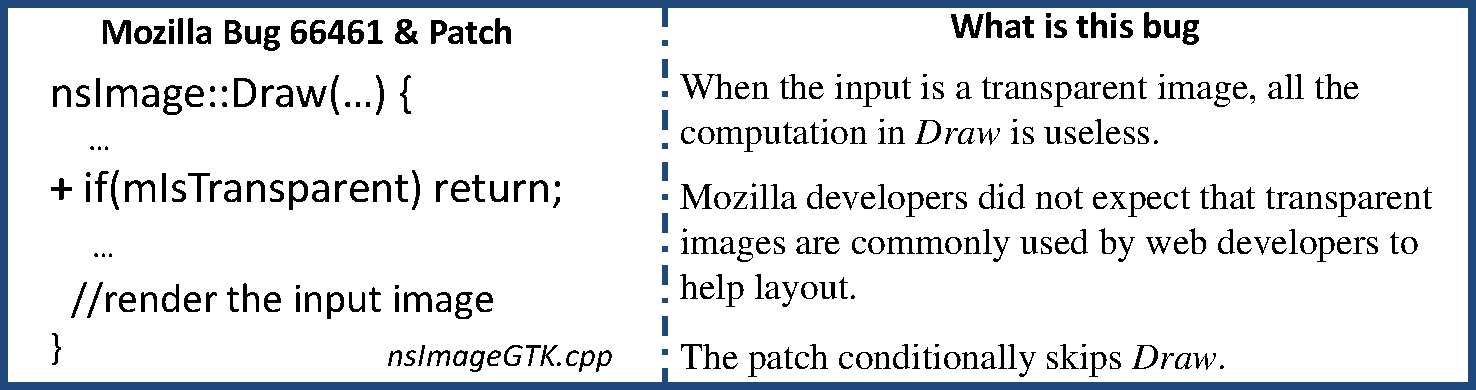
\includegraphics[width=3in]{figures/moz664614}
\caption{A Mozilla bug drawing transparent figures}
\label{fig:moz66461}
\end{center}
\end{figure}

\begin{figure}[t!]
\begin{center}
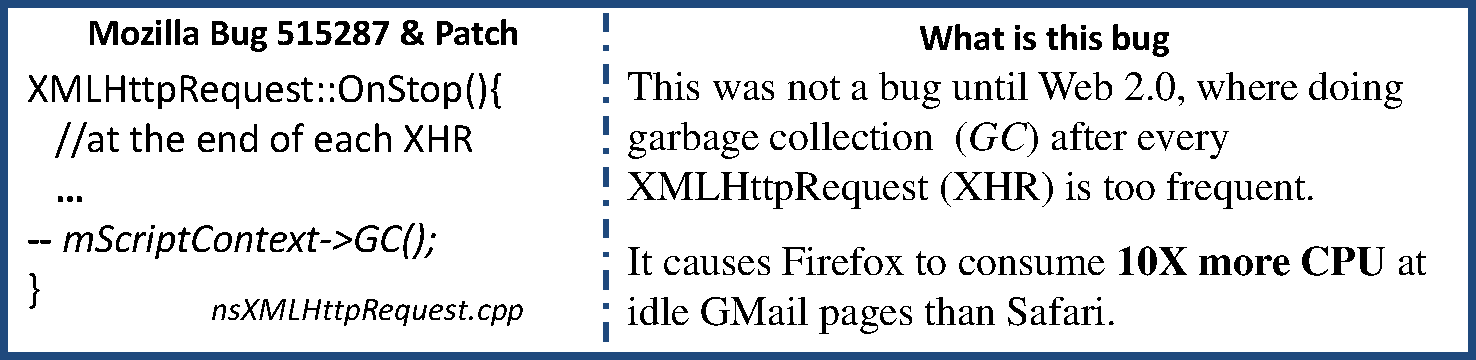
\includegraphics[width=3in]{figures/moz515287}
\caption{ {A Mozilla bug doing intensive GCs}}
\label{fig:moz515287}
\end{center}
\end{figure}

\begin{figure}[t]
\begin{center}
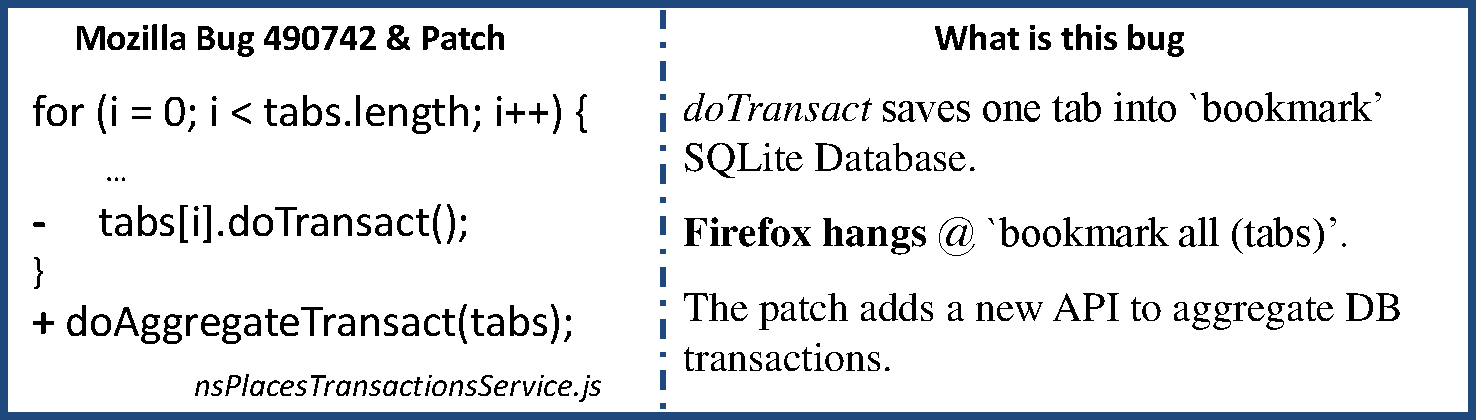
\includegraphics[width=3in]{figures/moz490742}
\caption{A Mozilla bug with un-batched DB operations}
\label{fig:uncoord2}
\end{center}
\end{figure}

\begin{figure}[t]
\centering
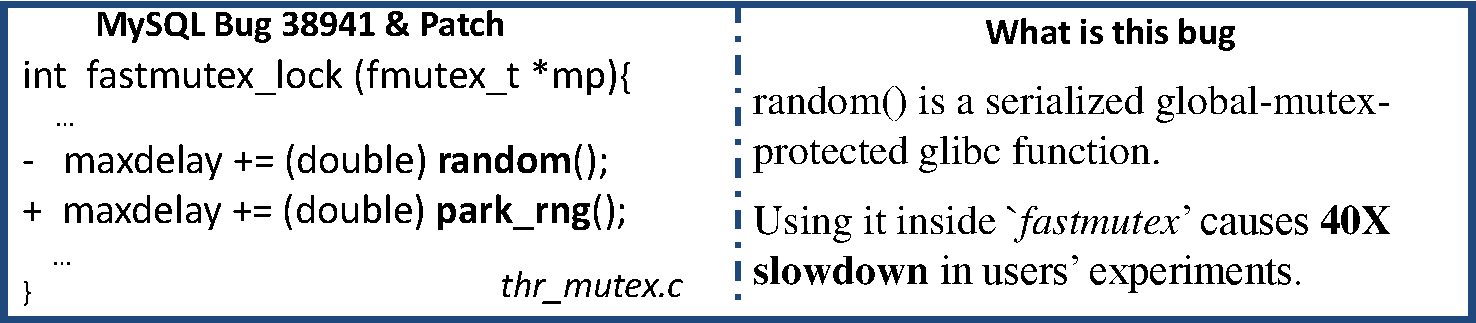
\includegraphics[width=3in]{figures/mysql38941}
\vspace{0.1in}
\caption{A MySQL bug with over synchronization}
\label{fig:mysql38941}
\end{figure}


\begin{figure}[t]
\centering
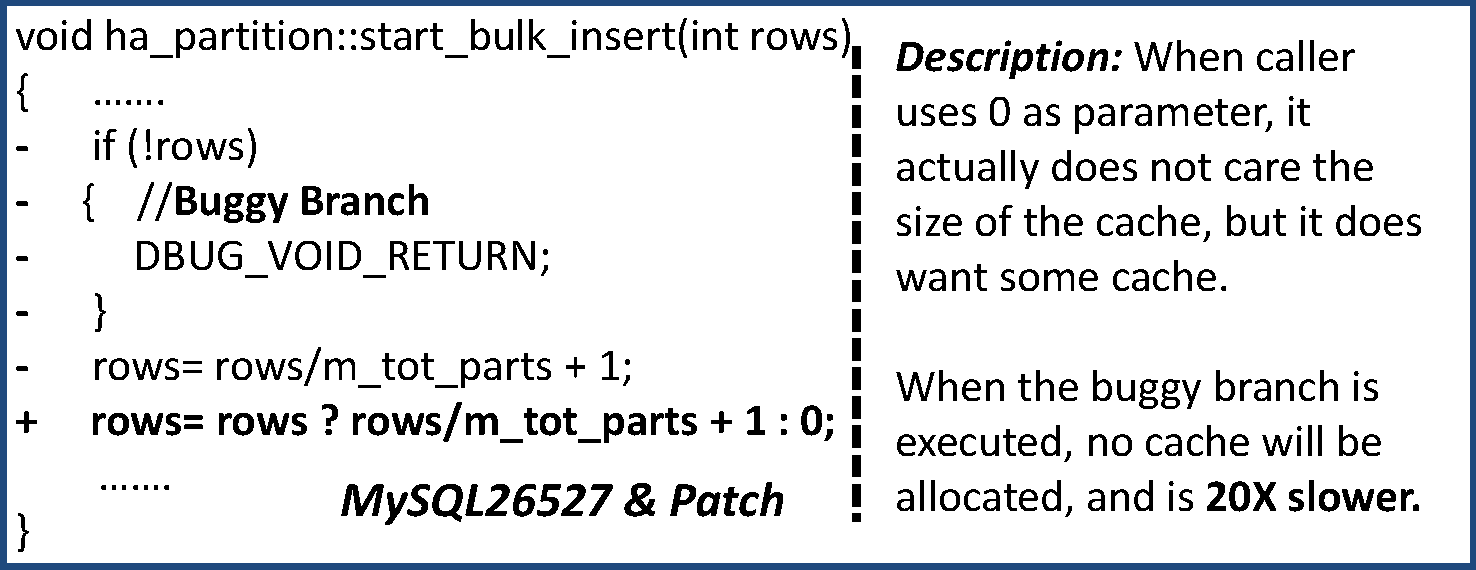
\includegraphics[width=3in]{figures/mysql26527}
\vspace{0.1in}
\caption{A MySQL bug without using cache}
\label{fig:mysql26527}
\end{figure}


\subsection{Root Causes of Performance Bugs}
\label{sec:taxonomy_howwaste}

There are a large variety of potential root causes for inefficient code, 
such as poorly designed algorithms, non-optimal data structures, cache-unfriendly data layouts, etc. 
Our goal here is not to discover previously unheard-of root causes, 
but to check whether there are common root-cause patterns among 
real-world performance bugs that bug detection and diagnosis work can focus on.

Our study shows that the majority of real-world performance bugs in our study are covered by only a couple of root-cause categories (Table~\ref{tab:root_cause}).

\underline{\it Wrong Branch Selection} 
A non-negligible portion of performance bugs are branch-related. 
There are three scenarios in which bugs in this category are triggered. 
In the first case, some slow code paths would be executed. 
For example, when Mozilla231300 is triggered, 
Firefox would use separate system calls to move files 
in the same directory one by one instead of using one system call to move them altogether. 
In the second case, some unnecessary work will be conducted. 
For example, when Mozilla258793 is triggered, 
Firefox will call draw functions for background figures, which do not exist. 
In the last case, some desired functionalities will be realized in an inefficient way, 
such as the {\it No Cache} example shown in Figure~\ref{fig:mysql26527}. 

\underline{\it Workless} 
Around one third of performance bugs are caused by workless codes. 
Buggy codes rarely generate results whenever executed, 
or they rarely generate results under bug-triggering inputs. 
Bugs in this category can be divided along two dimensions: 
according to different workless granularities, 
workless bugs can be divided into loop-related bugs and not loop-related bugs; 
based on whether semantic information is needed to judge whether codes are workless, 
bugs in this category can be divided into semantic workless, and non-semantic workless.
For example, inside the GC function, there is a loop to scan all heap objects 
and free objects with reference number 0. 
For the {\it Intensive GC} example in Figure~\ref{fig:moz515287}, this loop rarely deallocates objects. 
{\it Intensive GC} example  is loop-related and non-semantic workless.
{\it Transparent Draw} in Figure~\ref{fig:moz66461} is not loop-related, 
and we need semantic information to know that drawing a transparent figure is workless.

\underline{\it Redundancy} 
Redundancy means repeated work. 
Intuitively, we can remove repeated work and improve performance. 
According to different code granularity to observe redundant work, 
bugs in this category could be divided into redundant snippets, 
cross-iteration redundancy, and cross-loop redundancy.  
For example, in Chrome70153, 
both software and GPU will render the same video redundantly, 
and this bug is categorized as redundant snippets. 
In the {\it Bookmark All} example shown in Figure~\ref{fig:uncoord2}, 
Firefox will start, commit, and destroy a transaction for each tab in each iteration, 
and there is a lot of redundant work across different iterations. 
There are also bugs, for which redundant work is not inside one loop
but across different execution of the same loop, like Mozilla35294. 


\underline{\it Synchronization Issues}
Unnecessary synchronization that intensifies thread competition 
is also a common root cause, as shown in the {\it Slow Fast-Lock} bug (Figure~\ref{fig:mysql26527}). 
These bugs are especially common in server applications, contributing to 3 out of 15 Apache server bugs and 6 out of 26 MySQL server bugs.


\underline{\it Others}
There are also bugs that do not fall into above categories. 
For those bugs, developers find more efficient methods to optimize original codes. 
For example, in order to accelerate the startup of GPU process, Chrome developers use one extra thread to collect expensive GPU information. 
For MySQL14637, MySQL developers replace byte-wise parsing with four-byte-wise parsing to accelerate trimming blank characters from the end of a string. 

\begin{table*}[tb!]
\begin{adjustwidth}{-.5in}{-.5in}
\scriptsize
\centering
{

\begin{tabular}{lcccccc}
\toprule
\multicolumn{1}{c}{\bf Root Causes for Performance Bugs} &Apache&Chrome&GCC&Mozilla&MySQL&Total\\
\midrule
\multicolumn{1}{l}{Wrong Branch Selection: wrong branch selection to cause performance loss}
&2&0&1&6&7&16\\
\midrule
\multicolumn{1}{l}{Workless: not generate desired results}
&4&4&3&18&9&38\\
\midrule
\multicolumn{1}{l}{Redundancy: repeated work causing performance loss}
&13&3&3&6&2&27\\
\midrule
\multicolumn{1}{l}{Synchronization Issues: inefficient synchronization among threads}
&5&0&0&1&6&12\\
\midrule
\multicolumn{1}{l}{Others: all the bugs not belonging to the above four categories}
&4&3&4&6&7&24\\
\bottomrule

\end{tabular}
}
\end{adjustwidth}
\caption{Root cause categorization in Section~\ref{sec:taxonomy_howwaste}}
\label{tab:root_cause}
\end{table*}








%\underline{\it Control Flow of Performance Bugs}
%As we discussed earlier, there are performance bugs related to branch selection. 
%There are also bugs related loops, including bugs caused by workless loops, cross-iteration redundant bugs, cross-loop redundant bugs, 
%and some bugs categorized as Others. 
%Detailed numbers of control flow categorization for performance bugs 
%and user perceived performance bugs are shown in Table~\ref{tab:cfg} and Table~\ref{tab:cfg_user} respectively. 
%There are more than 80\% of user perceived performance bugs either related to branches or related to loops.
%Future performance bug diagnosis tools can focus on these two types of bugs.   






\section{How Performance Bugs Are Introduced}
\label{sec:char_introduce}

\begin{table*}[tb!]
\begin{adjustwidth}{-.5in}{-.5in}
\scriptsize
\centering
{
\begin{tabular}{lcccccc}
\toprule
\multicolumn{1}{c}{\bf How Performance Bugs Are Introduced} &Apache&Chrome&GCC&Mozilla&MySQL&Total\\
\midrule
\multicolumn{1}{l}{Workload Issues: {developers' workload assumption is wrong or out-dated}}
&13&2&5&14&7&41\\
\midrule
\multicolumn{1}{l}{API Issues: {misunderstand performance features of functions/APIs}}
&6&3&1&13&8&31\\
\midrule
\multicolumn{1}{l}{Others: all the bugs not belonging to the above two categories}
&6&5&5&10&13&39\\
\bottomrule

\end{tabular}
}
\end{adjustwidth}
\caption{How performance bugs are introduced in Sections~\ref{sec:char_introduce}}
\label{tab:intro}
\end{table*}

We have studied the discussion among developers in bug databases and checked the 
source code of different software versions to understand how bugs are introduced. 
Our study has particularly focused on the challenges faced by developers in writing 
efficient software, and features of modern software that affect the introduction
of performance bugs. 

Our study shows that developers are in a great need of tools that can help them 
avoid the following mistakes.

\underline{\it Workload Mismatch\ }
Performance bugs are most frequently introduced when 
developers' workload understanding does not match with the reality.

Our further investigation shows that the following challenges
are responsible for most workload mismatches.

Firstly, the input paradigm could shift {\it after}
code implementation. For example, the HTML standard change and new trends in 
web-page content led to {\it Transparent Draw} and
{\it Intensive GC}, shown
in Figure~\ref{fig:moz66461} and Figure~\ref{fig:moz515287}.

Secondly, software workload has become much more diverse and complex than 
before.
A single program, such as Mozilla, may face various types of workload issues:
the popularity of transparent figures on web pages led
to {\it Transparent Draw} 
in Figure \ref{fig:moz66461}; the high frequency of XMLHttpRequest led to
{\it Intensive GC}
in Figure \ref{fig:moz515287}; users' habit of not changing the default
configuration setting led to Mozilla110555. 

The increasingly dynamic and diverse workload of modern software will lead
to more performance bugs in the future.

\underline{\it API Misunderstanding\ }
The second most common reason is that
developers misunderstand the performance feature of certain
functions. This occurs for 31 bugs in our study.

Sometimes, the performance of a function is sensitive to the value of a
particular parameter, and developers happen to use performance-hurting values. 

Sometimes, developers use a function to perform task $i$, and are unaware of
an irrelevant task $j$ 
conducted by this function that hurts performance but not functionality. 
For example, MySQL developers did not know the synchronization inside
random and introduced the {\it Slow Fast-Lock} bug shown in 
Figure~\ref{fig:mysql38941}. 

Code encapsulation in modern software leads to many APIs with poorly 
documented performance features. 
We have seen developers explicitly complain about this issue 
\citep{apache45396}. It will lead to more performance bugs in the future.

\underline{\it Others\ }
Apart from workload issues and API issues, there are also other reasons behind
performance bugs. Interestingly,
some performance bugs are side-effects of functional bugs. For example, 
in Mozilla196994,
developers forgot to reset a busy-flag. This semantic bug causes an event 
handler to be constantly busy. As a result, a performance loss is the only 
externally visible 
symptom of this bug.

\underline{\it When a bug was not buggy\ }
An interesting trend is that 29 out of \allbugs bugs were not born buggy.
They became inefficient long after they were written due to workload shift,
such as that in {\it Transparent Draw} and {\it Intensive GC}
(Figures~\ref{fig:moz66461} and \ref{fig:moz515287}), 
and code changes in other part of the software, such as
that in Figure XX.
In Chrome70153, when GPU accelerator became available, software
rendering code became redundant.
Many of these bugs went through regression testing without being caught.



\section{How Performance Bugs Are Exposed And Perceived}
\label{sec:char_exp}


\begin{table*}[tb!]
\begin{adjustwidth}{-.5in}{-.5in}
\scriptsize
\centering
{
\begin{tabular}{lcccccc}
\toprule
\multicolumn{1}{c}{\bf How Performance Bugs Are Exposed} &Apache&Chrome&GCC&Mozilla&MySQL&Total\\
\midrule
\multicolumn{1}{l}{Always Active: almost every input on every platform can trigger this bug}
&2&3&0&6&4&15\\
\midrule
\multicolumn{1}{l}{Special Feature: need special-value inputs to cover specific code regions}
&19&6&11&22&18&76\\
\midrule
\multicolumn{1}{l}{Special Scale: need large-scale inputs to execute a code region many times}
&17&2&10&23&19&71\\
\midrule
\multicolumn{1}{l}{Feature+Scale: the intersection of Special Feature and Special Scale}
&13&1&10&15&13&52\\
\bottomrule
\end{tabular}
}
\end{adjustwidth}
\caption{How performance bugs are exposed in Section~\ref{sec:char_exp}}
\label{tab:exp}
\end{table*}

 

{\bf How to Expose Performance Bugs?} We define exposing a performance bug as causing a perceivably negative performance impact, 
following the convention used in most bug reports. Our study demonstrates several unique challenges for performance testing.

\underline{\it Always Active Bugs\ } 
A non-negligible portion of performance bugs are almost always active.
They are located at the start-up phase, the shutdown phase, or other places 
that are exercised by almost all inputs. 
They could be very harmful in the long term, because
they waste performance at every deployment site during every run of a program.
Many of these bugs were caught during comparison with other software
(e.g., Chrome vs. Mozilla vs. Safari).

Judging whether performance bugs have manifested is a unique challenge in 
performance testing.

\underline{\it Input Feature \& Scale Conditions\ } 
About two thirds of performance bugs need inputs with special features
to manifest. Otherwise, the buggy code units cannot be touched.
Unfortunately, this is not what black-box testing is good at.
Much manual effort will be needed to design test inputs, a problem
well studied by past research in functional testing \citep{KLEE,s2e}.


About two thirds of performance bugs need large-scale inputs to manifest in
a perceivable way. These bugs cannot be effectively exposed if 
software testing executes each buggy code unit only once,
which unfortunately is the goal of most functional testing.

Almost half of the bugs need inputs that have special features {\bf and} 
large scales to manifest. 
For example, to trigger the bug shown in Figure~\ref{fig:uncoord2}, the user
has to click `bookmark all' button (i.e., special feature) with many open
tabs (i.e., large scale).




\begin{table*}[tb!]
\begin{adjustwidth}{-.5in}{-.5in}
\scriptsize
\centering
{
\begin{tabular}{lcccccc}
\toprule
\multicolumn{1}{c}{\bf How Performance Bugs Are Perceived} &Apache&Chrome&GCC&Mozilla&MySQL&Total\\
\midrule
\multicolumn{1}{l}{Comparison in one code base}
&9&3&6&7&12&37\\
\midrule
\multicolumn{1}{l}{Comparison between different code bases}
&7&3&8&5&4&27\\
\midrule
\multicolumn{1}{l}{Not using comparison-based methods}
&3&1&1&9&2&16\\
\bottomrule
\end{tabular}
}
\end{adjustwidth}
\caption{How performance bugs are perceived in Section~\ref{sec:char_exp}}
\label{tab:cmp}
\end{table*}

{\bf How to Perceive Performance Bugs?}
The majority of user-perceived performance bugs are noticed and reported by comparison-based methods. 
Comparison can be divided into comparison within one code base
and comparison between different code bases. 
It is possible that one bug is reported by more than one comparison-based methods. 

\underline{\it One Code Base} In this case, users use at least one good and one bad input 
to run the same program, compare the performance, and notice performance loss. 
Comparison in this category involves comparison between different input sizes, 
comparison between different execution environments, 
and comparison between similar inputs. 

\underline{\it Different Code Bases} 
Users use one input.
Performance difference between different software versions or different applications exposes performance problems to users. 
Examples for different types of comparison are shown in Table~\ref{tab:example}.

\underline{\it Not Using Comparison-based Methods}
Users directly describe performance impact for these bugs, 
such as ``froze to crawl'' for Mozilla299742 and ``It’s very slow'' for Mozilla227361. 




\begin{table*}[tb!]
\scriptsize
\centering
{
\begin{tabular}{ll}
\toprule
{\bf Comparison} & {\bf Example}\\
\midrule 
\multirow{3}{0.8in}{Applications} & {\bf Mozilla515287:} ``When running several Gmail instances in open tabs on my laptop (OS X), the \\
& CPU utilization is 15-20\% even while just idling. This has been tested with a blank profile, and no \\
& extensions. On Safari, the same open windows are at ~1.5\% CPU utilization."\\
\midrule
\multirow{3}{0.8in}{Versions} & {\bf GCC12322:} ``The GCC-3.4 development snapshots take 5x or 6x as long to compile the \\
& computed-goto heavy core\_ops\_cg.c in Parrot. GCC-3.3 compiles this file in about five or six \\
& minutes on my slow  machine - GCC-3.4 takes 30 or more minutes."\\
\midrule
\multirow{2}{0.8in}{Environments} & {\bf MySQL48429:} The performance of some sql with "group by" on partitioned table is very bad.\\
&Users provide the query time on partitioned table and unpartitioned table. \\
\midrule
\multirow{2}{0.8in}{Sizes} & {\bf Mozilla104328:} ``On my windows machine my accumulated ~250 bookmarks takes about 2.5\% of  \\
&my normal 6 second startup. With a 1111 bookmark file my startup takes 42 seconds."\\
\midrule
\multirow{2}{0.8in}{Similar Inputs} & {\bf Mozilla336944:} ``Happens on https://bugzilla.mozilla.org/ ... hogging the CPU the whole time\\
& (2-3 minutes or more instead of ~30 seconds for http://tinyurl.com/msj4y).'' \\
\bottomrule
\end{tabular}
%\caption{Examples for Different Types of Comparison(this table needs to be changed)}
\caption{Examples of different types of comparison}
\label{tab:example}
}
\end{table*}

\subsection{How Performance Bugs Are Fixed}
\label{sec:char_fix}

\begin{table*}[tb!]
\begin{adjustwidth}{-.5in}{-.5in}
\scriptsize
\centering
{

\begin{tabular}{|l|c|c|c|c|c|c|}
\toprule
\multicolumn{1}{|c|}{\bf Granularity for Performance Bugs} &Apache&Chrome&GCC&Mozilla&MySQL&Total\\
\midrule
\multicolumn{1}{|l|}{Performance bugs happening at function boundaries}
&22&8&4&29&18&81\\
\midrule
\multicolumn{1}{|l|}{Performance bugs not happening at function boundaries}
&3&2&7&7&10&29\\
\bottomrule

\end{tabular}
}
\end{adjustwidth}
\caption{Granularity categorization for performance bugs in Section~\ref{sec:char_fix}}
\label{tab:location}
\end{table*}

We find that most performance bugs happen at call sites, and they are fixed by changing the usage of function calls, 
such as replacing old call sequences with new call sequences, conditionally or unconditionally skipping buggy functions or changing parameters, and so on. 
For example, {\it Transparent Draw} (Figure~\ref{fig:moz66461}), {\it Intensive GC} (Figure~\ref{fig:moz515287}), 
{\it Bookmark All} (Figure~\ref{fig:uncoord2}), and
{\it Slow Fast-Lock} (Figure~\ref{fig:mysql38941}) are all fixed by changing function call usage.
This is probably because developers and compilers have already done a good job in optimizing code within each procedure. 
Therefore, future work to detect, diagnose and fix performance bugs should allocate more effort at call sites and procedure boundaries. 

There are also 29 bugs not fixed by changing function call usage. 
These bugs mainly arise from two scenarios. 
In one scenario, the buggy code unit itself does not directly waste performance. 
Instead, its impact propagates to other places in the software and causes performance loss there. 
For example, the {\it No Cache} (Figure~\ref{fig:mysql26527}) 
bug happens when MySQL mistakenly does not allocate cache. 
This operation itself does not take time, but it causes performance loss later. 
The second scenario is to optimize code units inside functions, like MySQL14637, whose patch replaces byte-wise parsing with
four-byte-wise parsing to accelerate trimming blank characters from the end of a string.


\begin{table*}[tb!]
\begin{adjustwidth}{-.5in}{-.5in}
\scriptsize
\centering
{
\begin{tabular}{|l|c|c|c|c|c|c|}
\toprule
\multicolumn{1}{|c|}{\bf How to Fix Performance Bugs} &Apache&Chrome&GCC&Mozilla&MySQL&Total\\
\midrule
\multicolumn{1}{|l|}{Change Condition: {a condition is added or modified} }
&1&4&7&14&10&36\\
\midrule
\multicolumn{1}{|l|}{In-place Call Change: {replace call sequences in the exact same place} }
&9&1&1&8&8&27\\
\midrule
\multicolumn{1}{|l|}{Memorization: {reuse results from previous computation}}
&9&0&3&3&3&18\\
\midrule
 \multicolumn{1}{|l|}{Batch: {batch computation to eliminate  redundancy}}
&4&3&0&6&1&14\\
\midrule
\multicolumn{1}{|l|}{Others: all the bugs not belonging to the above four categories}
&2&2&1&5&6&16\\
\bottomrule
\end{tabular}
}
\end{adjustwidth}
\caption{How to fix performance bugs in Section~\ref{sec:char_fix}}
\label{tab:fix}
\end{table*}


There are four common strategies in fixing performance bugs, as shown in Table~\ref{tab:fix}.

\underline{\it Change Condition} The most common fix strategy is {\it Change Condition}. 
It is used in 36 patches, in which code units that do not always generate useful 
results are conditionally skipped, 
a fast path is changed to be executed, or the same functionality is realized in a more efficient way. 
For example, Draw is conditionally skipped to fix {\it Transparent Draw} (Figure~\ref{fig:moz66461}), 
and cache will be used to fix {\it No Cache} (Figure~\ref{fig:mysql26527} ).

\underline{\it In-place Call Change} The second most common strategy is {\it In-place Call Change}. 
In this strategy, developers replace or reorganize the call sequence in the exact same place. 
The performance gain can be achieved whenever changed codes are executed. 
For example, in order to fix Mozilla103330, 
developers replace the setLength and Append call combination with Assign.

\underline{\it Memorization} fixes 18 bugs by reusing results 
from previous calculations. 
For example, in order to fix Mozilla409961, 
developers move do\_QueryInterface outside the buggy loop, instead of calling it in each iteration.  

\underline{\it Batch} strategy is used in 14 patches. 
For example, {\it Bookmark All} in Figure~\ref{fig:uncoord2} is fixed by this strategy.   

\underline{\it Are patches complicated?}
Most performance bugs in our study can be fixed through simple changes. 
In fact, 42 out of 110 bug patches contain five or fewer lines of code changes. 
The median patch size for all examined bugs is 8 lines of code.
The small patch size is a result of the above fixing strategies.
Many change condition patches are small. Most in-place call change, memorization, and batch patches do not require implementing new function calls.







\section{Other Characteristics}
\label{sec:char_life}
{\bf Life Time\ } We chose Mozilla to investigate the life time of performance bugs, 
due to its convenient CVS query interface.
We consider a bug's life to have started when its buggy code
was first written. The 36 Mozilla bugs in our study
took 935 days on average to get discovered, and another 140 days on average
to be fixed.
For comparison, we randomly sampled 36 functional bugs from Mozilla.
These bugs took 252 days on average to be discovered, which is much shorter 
than that of performance bugs in Mozilla.
These bugs took another 117
days on average to be fixed, which is a similar amount of time with those
performance bugs.

{\bf Location\ } For each bug, we studied the location of its
minimum unit of inefficiency. We found that 
over three quarters of bugs are
located inside either an input-dependent loop or an input-event handler. 
For example, the buggy code in Figure~\ref{fig:moz515287}
is executed at every XHR completion.
The bug in Figure~\ref{fig:moz66461} wastes performance
for every transparent image on a web page.
In addition, about half performance bugs involve I/Os or 
other time-consuming system calls. 
There are a few bugs whose buggy code units only execute once or twice
during each program execution. For example, the Mozilla110555 bug wastes
performance while processing exactly two fixed-size
default configuration files,
userChrome.css and userContent.css, during the startup of a browser.

{\bf Correlation Among Categories}
Following previous empirical studies \citep{LiASID06}, we use a statistical 
metric {\it lift} to study the correlation among characteristic categories.
The {\it lift} of category A and category B, denoted as {\it lift(AB)}, 
    is calculated 
as $\frac{P(AB)}{P(A)P(B)}$, where P(AB) is the probability of a bug belonging 
to both categories A and B. When {\it lift(AB)} equals 1,   
category A and category B are independent of each other.
When {\it lift(AB)} is greater than 1, categories A and B are 
positively correlated: when a bug belongs to A, it likely
also belongs to B. The larger the {\it lift} is, the more positively A and B
are correlated.
When {\it lift(AB)} is smaller than 1, A and B are negatively
correlated: when a bug belongs to A, it likely does not belong to B.
The smaller the {\it lift} is, the more negatively A and B are correlated.

Root cause categories are highly correlated with fix strategies. 
Among all correlations, the redundant root cause and the memorization fix strategy are 
the most positively correlated with a 3.62. 
The wrong branch selection root cause is strongly correlated with the change condition 
fix strategy with a 2.48 lift. The redundant root cause and the batch fix strategy are the third 
most positively correlated pair with a 2.32 lift. 
On the other hand, the wrong branch selection root cause has the most negative correlation 
with in-place call Change, memorization and batch bug-fix strategies. 
Their lifts are all 0. 
Among all other correlations, the workload mismatch introducing reason and the batch fix strategy 
are positively correlated with a 1.91 lift.


{\bf Server Bugs vs. Client Bugs}
Our study includes 41 bugs from server applications and 69 bugs from client 
applications. To understand whether these two types of bugs have different 
characteristics, we apply chi-square test
\citep{chisquared} to each
category listed in Table~\ref{tab:root_cause}, Table~\ref{tab:intro}, Table~\ref{tab:exp} and Table~\ref{tab:fix}.
We choose 0.01 as the significance level of our chi-square test. 
Under this setting, if we conclude that server and client bugs have different
probabilities of falling into a particular characteristic category, 
this conclusion only has a 1\% probability to be wrong. 

We find that, among all the categories listed in Table~\ref{tab:root_cause}, Table~\ref{tab:intro}, Table~\ref{tab:exp} and Table~\ref{tab:fix},
only the synchronization issues category
is significantly different between server bugs 
and client bugs ---
synchronization issues have caused 22\% of server bugs and only 
4.3\% of client bugs.


%\subsection{Lessons from Our Study}
%\label{sec:lessons}

\section{Guidance for My Thesis Work}


{\bf Bug Detection}
Our study provides several motivation for our rule-based bug detection work, 
which will be discussed in detail in Section~\ref{sec:detect}. 
Most performance bugs loss performance at function-call sites (Section~\ref{sec:char_fix}), 
and more than one fourth of performance bugs are introduced by misunderstanding API (Section~\ref{sec:char_introduce}). 
We could detect similar inefficient call usage to find new bugs. 
Because some performance bugs are always active (Section~\ref{sec:char_exp}), 
performance bugs cannot be modeled as rare events.
Automatically inferring efficiency rules may not be feasible for performance bugs. 
Patches for performance bugs are simple (Section~\ref{sec:char_fix}), and they follow limited fix strategies. It is feasible to extract efficiency rules from these patches. 

{\bf Bug Diagnosis}
Our study also provides guidance for our comparison-based performance 
bug diagnosis work (Section~\ref{sec:inhouse}). 
Users use comparison-based methods to notice performance loss (Section~\ref{sec:char_exp}), 
and we could borrow the same philosophy in designing our diagnosis systems. 
Most performance loss happens at function boundaries (Section~\ref{sec:char_fix}), 
and we could utilize this information to infer root causes for performance bugs. 
The patch for performance bugs follow limited fix strategies (Section~\ref{sec:char_fix}), 
and these strategies are highly related to root causes (Section~\ref{sec:char_life}). 
It is feasible for our diagnosis systems to give out fix suggestions to developers automatically. 



\section{Guidance for Future Work}

{\bf Comparison with Functional Bugs\ }
There are several interesting comparisons between performance and functional
bugs. (1)
The distribution of performance-failure rates over software life time
follows neither the bathtub model of
hardware errors nor the gradually maturing model of functional bugs, because
performance bugs have long hiding periods (Section \ref{sec:char_life}) 
and can emerge from non-buggy 
places when software evolves (Section \ref{sec:char_introduce}).
(2) Unlike functional bugs, performance bugs cannot always be modeled as 
rare events, because some of them are always active 
(Section \ref{sec:char_exp}).
(3) The percentage of synchronization problems among
performance bugs in our study is higher than the percentage of synchronization
problems among functional bugs in a previous study for
a similar set of applications~\citep{LiASID06} (Section \ref{sec:taxonomy_howwaste}).

{\bf Annotation Systems\ }
Annotation systems are used in many software development environments
\citep{msdnannot,linuxannot}. Unfortunately, they mainly communicate
functionality information.%, but not performance-related information.

Our study calls for performance-aware annotation systems
\citep{perfassert1,perfassert2}
that help developers maintain and communicate APIs' performance features
and workload assumptions (Section \ref{sec:char_introduce}).
%Therefore, developers can make informed decisions when they face large and 
%varied APIs. 
Simple support such as warning about the existence of locks in
a library function, specifying the complexity of a function, and
indicating the desired range of a performance-sensitive parameter
%or specifying the complexity of an API 
can go a long way in avoiding performance bugs.
Recent work that automatically calculates function complexity is
also promising \citep{gulwani.popl2009}.

{\bf Testing\ }
Regression testing and change-impact analysis have to
consider workload changes and performance impacts, because new performance bugs
may emerge from old code
(Section \ref{sec:char_introduce}).

Performance testing can be improved if its input
design combines smart input-generation techniques used in functional testing
\citep{KLEE, dart} with an emphasis on large scale
(Section~\ref{sec:char_exp}).

Expressing performance oracles and judging whether performance bugs have 
occurred are critical challenges in performance testing 
(Section~\ref{sec:char_exp}). Techniques that can smartly compare performance
numbers across inputs and automatically discover the existence of 
performance problems are 
desired.

{\bf Future Directions}
One might argue that performance sometimes needs
to be sacrificed for better productivity and functional correctness. However,
the fact that we can often achieve significant performance improvement through
only a few lines of code change motivates future research to pay more
attention to performance bugs (Section~\ref{sec:char_fix}).
Our study suggests 
that the workload trend and API features of modern software will lead
to more performance bugs in the future (Section~\ref{sec:char_introduce}).
In addition, our study observes a significant portion of synchronization-related
performance bugs in multi-threaded software. There will be more bugs of this
type in the multi-core era. Beyond research discussed in this proposal, we think 
that there are still several potential directions to combat performance bugs.

Finally, our observations have been consistent across old software and new 
software (Chrome), old bugs (27 pre-2004 bugs) and new bugs (44 post-2008 bugs).
Therefore, we are confident that these lessons will be useful at least 
for the near
future.


